\section{linear model analysis}

The continue state space model where $u=V$ (voltage on the motor) and x=$[\theta \ \alpha \  \dot{\theta} \ \dot{\alpha} ]$. The system can only directly measure $\theta$ and $\alpha$, so these determine the matrix C and D.
$$
\begin{cases}
\dot{x}=Ax+Bu \\
y=Cx+Du
\end{cases}
$$

$$
A=
\begin{bmatrix}
0 & 0 & 1 & 0 \\
0 & 0 & 0 & 1 \\
0 & 40.7 & -12.2 & 0 \\
0 & 38.6 & -4.7 & 0 
\end{bmatrix}
B=
\begin{bmatrix}
0 \\
0 \\
23.3 \\
8.3
\end{bmatrix}
C=
\begin{bmatrix}
1 & 0 & 0 & 0\\
0 & 1 & 0 & 0
\end{bmatrix}
D=
\begin{bmatrix}
0 & 0
\end{bmatrix}
$$

\begin{figure}[H]
	\centering
	\begin{subfigure}[b]{0.45\textwidth}
		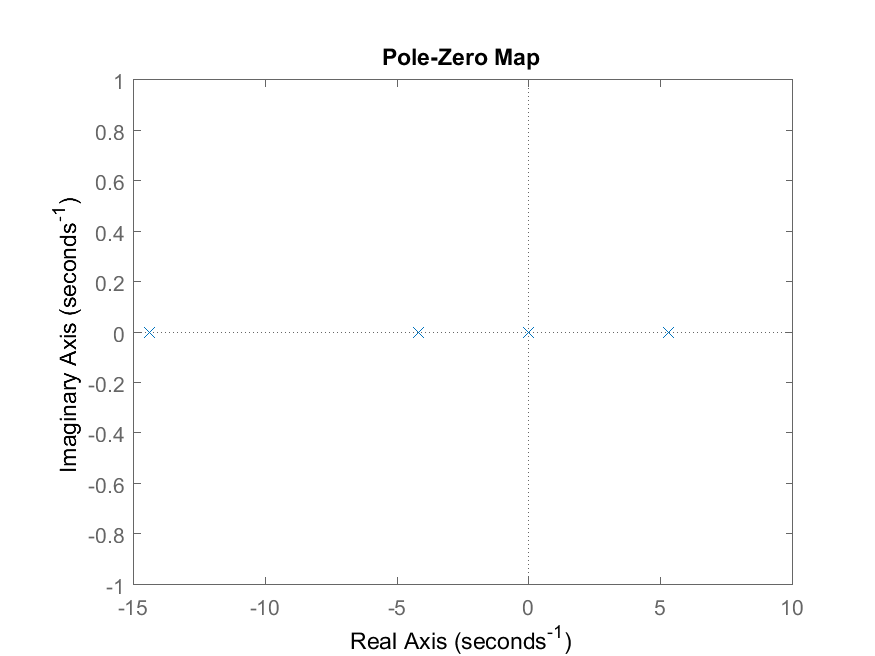
\includegraphics[width=\textwidth]{./part1_analysis/zplot.png}
		\caption{plot of poles and zeros}
	\end{subfigure}
	\begin{subfigure}[b]{0.45\textwidth}
		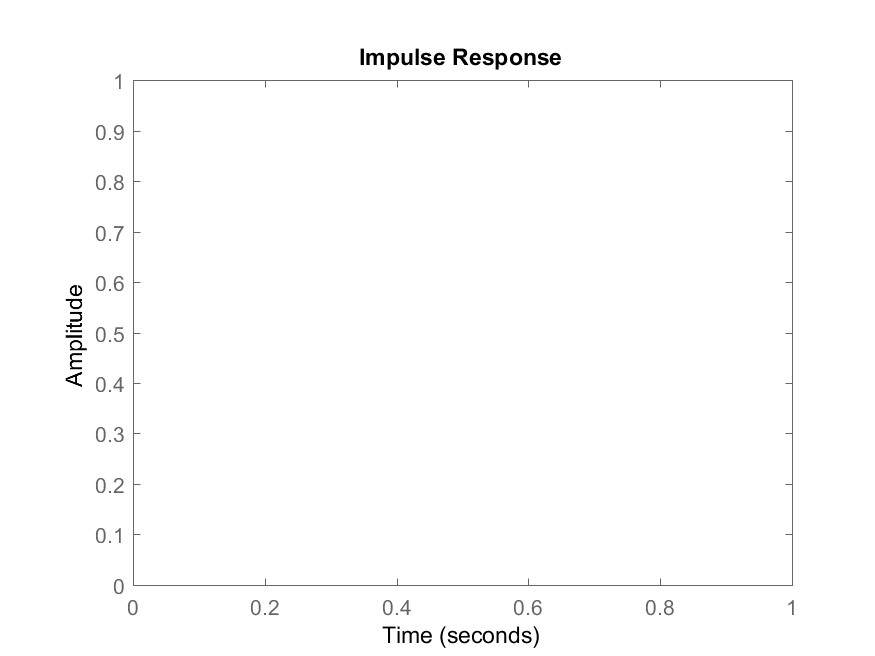
\includegraphics[width=\textwidth]{./part1_analysis/impulse.png}
		\caption{impulse response}
	\end{subfigure}
	\begin{subfigure}[b]{0.45\textwidth}
		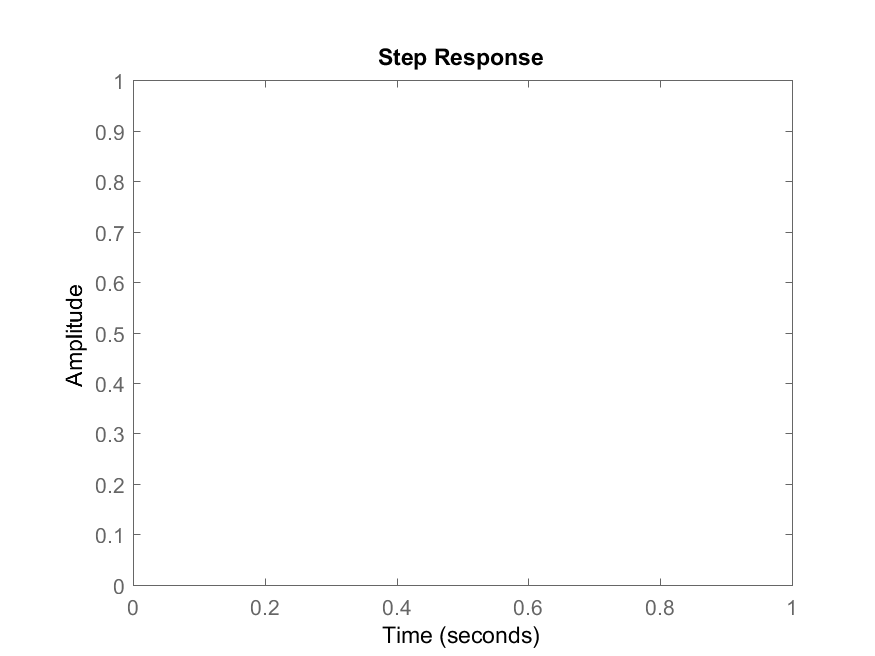
\includegraphics[width=\textwidth]{./part1_analysis/step.png}
		\caption{step response}
	\end{subfigure}
\end{figure}